\documentclass[a4paper 12pt]{article}

\usepackage[utf8]{inputenc}
\usepackage[T1]{fontenc}
\usepackage{mathptmx}
\usepackage{textcomp}
\usepackage[UKenglish]{babel}
\usepackage{amsmath, amssymb}
\usepackage{float}
\usepackage{xcolor}
\definecolor{backcolor}{rgb}{0.95,0.95,0.92}
\definecolor{codegreen}{rgb}{0,0.6,0}
\definecolor{codepurple}{rgb}{0.58,0,0.82}
\usepackage{listings}
\lstdefinestyle{code}{
	backgroundcolor=\color{backcolor},
	commentstyle=\color{codegreen},
	keywordstyle=\color{magenta},
	stringstyle=\color{codepurple},
	showspaces=false,
	showstringspaces=false,
	breaklines=true
}
\lstset{style=code}
\usepackage[hidelinks]{hyperref}
\hypersetup{
	colorlinks=false
}
\usepackage[style=ieee]{biblatex}
\bibliography{sources/biblio}
\renewcommand{\baselinestretch}{1.5}

\setlength{\parindent}{0pt}
\setlength{\parskip}{1em}

% figure support
\usepackage{import}
\usepackage{xifthen}
\pdfminorversion=7
\usepackage{pdfpages}
\usepackage{transparent}
\newcommand{\incfig}[1]{%
	\def\svgwidth{\columnwidth}
	\import{./figures/}{#1.pdf_tex}
}

\pdfsuppresswarningpagegroup=1

\begin{document}
\hypersetup{pageanchor=false}
\begin{titlepage}
  \begin{center}

    \textsc{\LARGE Dublin City University}\\[1cm]
    \textsc{\Large Electronic and Computer Engineering}\\[0.5cm]

    {\LARGE \bfseries Title\\[0.4cm]}
    {\Large \bfseries Subtitle\\[0.4cm]}

    \begin{figure}[H]
	
\includegraphics{images/Dcu-logo.png}
	\centering
    \end{figure}

    \vskip 2cm
    \emph{Author}\\[0.1cm]
    \noindent\makebox[\textwidth]{%
      \begin{tabular}{ll}%
        Michael Lenehan & michael.lenehan4@mail.dcu.ie \\
	Student Number: & 15410402 \\
    \end{tabular}}\\[0.1cm]

    \vfill

    % Bottom of the page
    % Probably replaced with date of deadline
    {\large{xx/xx/20xx}}

  \end{center}
\end{titlepage}

\hypersetup{pageanchor=true}
\pagenumbering{alph}
\thispagestyle{plain}
\begingroup
\renewcommand{\cleardoublepage}{}
\renewcommand{\clearpage}{}

\LARGE{Declaration}

\endgroup

\vskip 1cm

I declare that this material, which I now submit for assessment, is entirely my
own work and has not been taken from the work of others, save and to the extent
that such work has been cited and acknowledged within the text of my work. I
understand that plagiarism, collusion, and copying are grave and serious
offences in the university and accept the penalties that would be imposed should
I engage in plagiarism, collusion or copying. I have read and understood the
Assignment Regulations set out in the module documentation. I have identified
and included the source of all facts, ideas, opinions, and viewpoints of others
in the assignment references. Direct quotations from books, journal articles,
internet sources, module text, or any other source whatsoever are acknowledged
and the source cited are identified in the assignment references. This
assignment, or any part of it, has not been previously submitted by me or any
other person for assessment on this or any other course of study.

I have read and understood the DCU Academic Integrity and Plagiarism at
\url{https://www4.dcu.ie/sites/default/files/policy/1%20-%20integrity_and_plagiarism\_ovpaa_v3.pdf}
and IEEE referencing guidelines found at
\url{https://loop.dcu.ie/mod/url/view.php?id=448779}.

\vskip 1cm
Signed: \underline{\ \ \ \ \ \ \ \ \ \ \ \ \ \ \ \ \ \ \ \ \ \ \ \ \ \ \ \ \ \ \
\ \ \ \ \ \ } \hspace{20mm}Date: \underline{19/03/2020}

\hspace*{0mm}\phantom{Signed:}Michael Lenehan

\pagebreak

\pagenumbering{arabic}
\tableofcontents
\clearpage
\section{Question 1}
In order to draw the feasible region, the following information is required:

\begin{align*}
	4x + y &\le 5 \\
	\therefore \text{Intersects axis at} (0,5) &\text{and} (1.25,0) \\
	5x - 2y &\le 3 \\
	\therefore \text{Intersects axis at} (0,-1.5) &\text{and} (0.6, 0) \\
	y &\le 3 \\
	\therefore \text{A line parallel to the x-axis at} y &= 3 \\
\end{align*}

It is also given that the feasible region occurs in the quadrant greater than
$x=-1$ and  $y=-1$.

\begin{figure}[H]
	\centering
	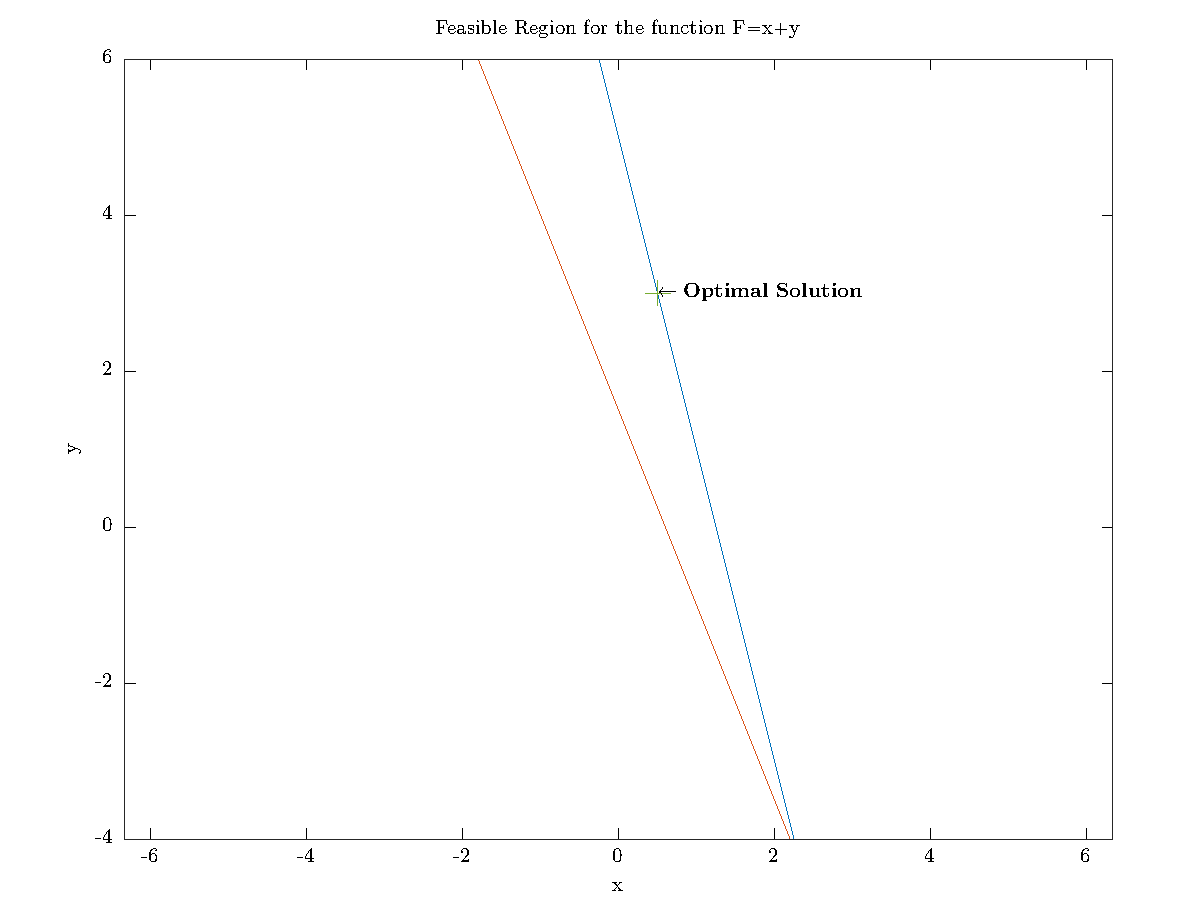
\includegraphics[width=\textwidth]{images/Q1}
	\caption{Feasible region for Q1}
	\label{fig:images-Q1}
\end{figure}

The maximum value is found to be at the point (0.5, 3.0).

If the objective function is changed to: minimise: $F=x$, the solution would be
(-1, 0), as the minimum value of x satisfies the objective function.

\section{Question 2}
\subsection{Part 1}

The following figure shows the block diagram of traffic flows/overflows within
the system. The A values ($A_{micA}$, $A_{micB}$, $A_{micC}$, $A_{mac}$, represent the
``Offered Load'' to the cells (Micro Cell A, Micro Cell B, Micro Cell C, Macro
Cell) respectively. $N_{mic}$ represents the number of channels in the micro
cells, while  $N_{mac}$ represents the number of channels in the macro cell. The
``Offered Load'' for the Overflow is represented by $A^*$, with the number of
channels represented by $N_{mac} + N^*$.

\begin{figure}[H]
	\centering
	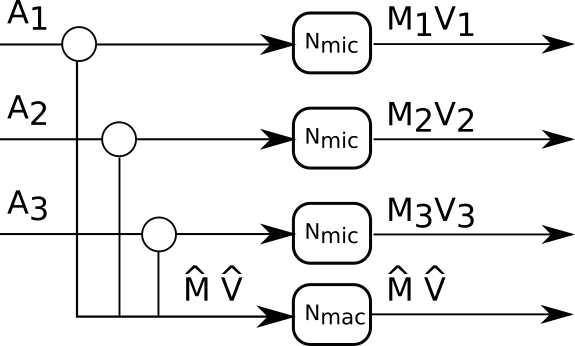
\includegraphics[width=0.8\textwidth]{images/Q6}
	\caption{Traffic Flows/Overflows Block Diagram}
	\label{fig:images-Q6}
\end{figure}

\subsection{Part 2}

The following table shows the Transition Probability Matrix for the process.

\begin{table}[H]
	\centering
	\caption{Transition Probability Matrix}
	\label{tab:label}
	\begin{tabular}{|c|c|c|c|c|c|}
		\hline
		0 & 1 & 2 & 3 & 4 & \ldots \\
		\hline
		0 & 0.5 & 0.5 & 0 & 0 & \ldots \\
		0 & 0 & 0.5 & 0.5 & 0 & \ldots \\
		0 & 0 & 0 & 0.5 & 0.5 & \ldots \\
		0 & 0 & 0 & 0 & 0.5 & 0.5 \\
		\hline
	\end{tabular}
\end{table}

\subsection{Part 3}

The minimum cost of the system is 102 cost units. This cost
corresponds to 24 Micro Cell Channels at 1 cost unit per channel, and 78 Macro
Cell Channels at 3 cost units per channel.

The figure below shows the Total System cost versus the number of Micro Cell
channels. The cost decreases to 102 up to 24 Micro Cell Channels, and increases
past this value.

\begin{figure}[H]
	\centering
	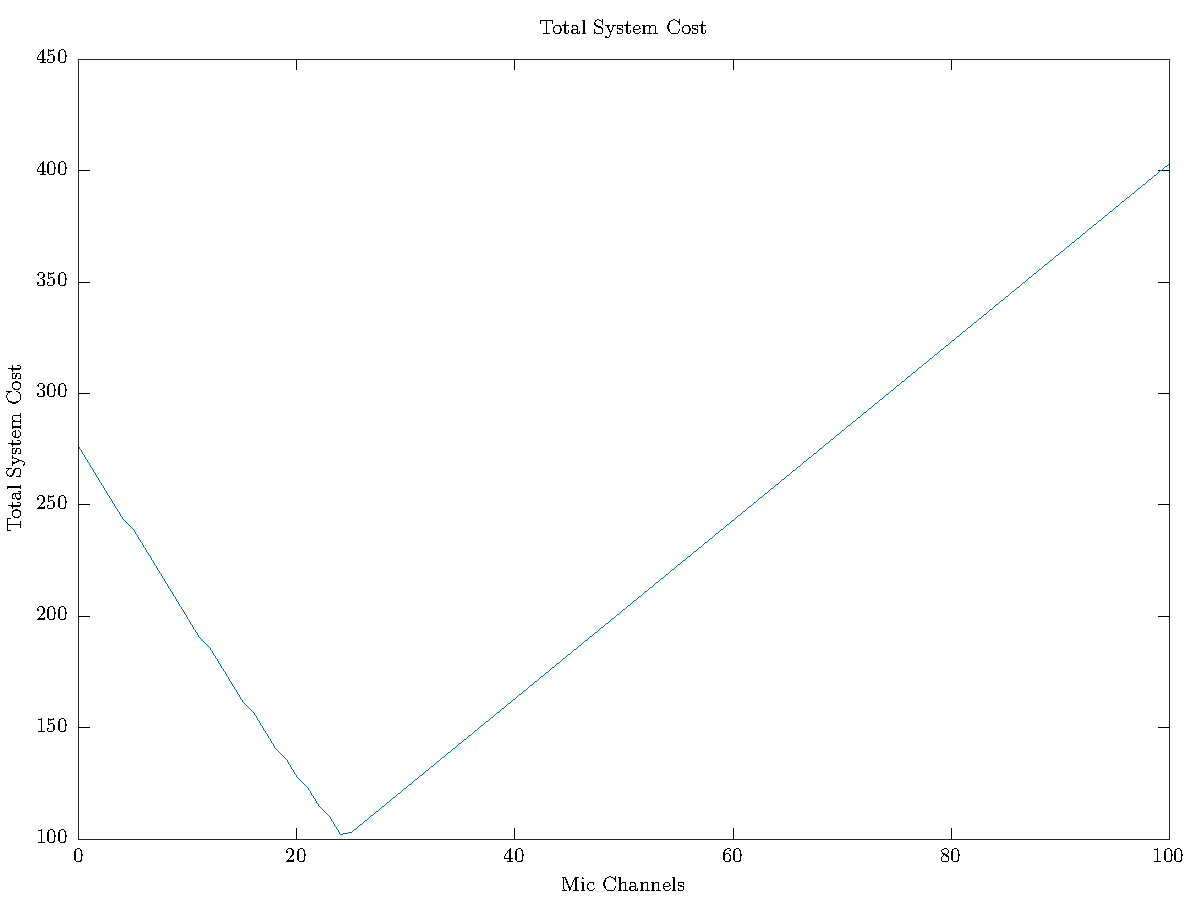
\includegraphics[width=0.8\textwidth]{code/Q6/Q6}
	\caption{Total System Cost vs. Micro Cell Channels}
	\label{fig:code-Q6-Q6}
\end{figure}

The following octave code shows the GNU-Octave implementation of the presented
problem. In order to calculate the minimum cost, the calculations described in
Part 2 are executed for increasing values of Micro Cell and Macro Cell Channels.
The blocking probability of each micro cell is calculated using the loops
current micro cell channel number and each cells respective offered load. These
blocking probabilities can be used to find the mean and variance for each cell.

A nested loop increments through the number of macro cell channels, calculating
the blocking probability, mean, and variance of the directly accessed macro
cell. The offered load and number of channels for the overflow channel is given
by using Rapps approximations on the total means and variances for the micro and
macro cells.

Using the offered load and number of channels for the overflow channel from
Rapps approximations, the overall blocking probability can be calculated. This
loop executes until the blocking probability drops below the required
QoS value of 1%.

For all calculations of blocking probabilities, the iterative method for
Erlang-B is used.

\lstinputlisting[language=octave]{code/Q6/q6.m}

\section{Question 3}
\subsection{Part 1}

The following figure shows the block diagram of traffic flows/overflows within
the system. The A values ($A_{micA}$, $A_{micB}$, $A_{micC}$, $A_{mac}$, represent the
``Offered Load'' to the cells (Micro Cell A, Micro Cell B, Micro Cell C, Macro
Cell) respectively. $N_{mic}$ represents the number of channels in the micro
cells, while  $N_{mac}$ represents the number of channels in the macro cell. The
``Offered Load'' for the Overflow is represented by $A^*$, with the number of
channels represented by $N_{mac} + N^*$.

\begin{figure}[H]
	\centering
	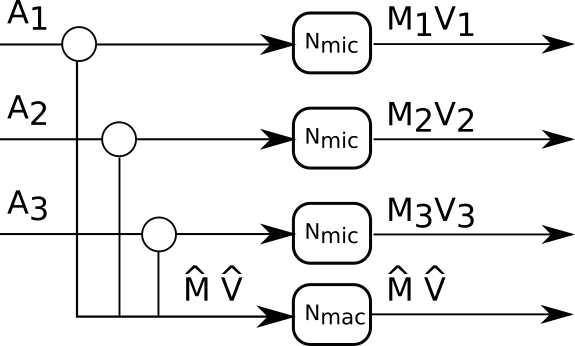
\includegraphics[width=0.8\textwidth]{images/Q6}
	\caption{Traffic Flows/Overflows Block Diagram}
	\label{fig:images-Q6}
\end{figure}

\subsection{Part 2}

The following table shows the Transition Probability Matrix for the process.

\begin{table}[H]
	\centering
	\caption{Transition Probability Matrix}
	\label{tab:label}
	\begin{tabular}{|c|c|c|c|c|c|}
		\hline
		0 & 1 & 2 & 3 & 4 & \ldots \\
		\hline
		0 & 0.5 & 0.5 & 0 & 0 & \ldots \\
		0 & 0 & 0.5 & 0.5 & 0 & \ldots \\
		0 & 0 & 0 & 0.5 & 0.5 & \ldots \\
		0 & 0 & 0 & 0 & 0.5 & 0.5 \\
		\hline
	\end{tabular}
\end{table}

\section{Question 4}
\begin{align*}
	\text{Distribution of the Waiting Time:} \\
	F_{W}(T) &= 1 - \rho e^{-\mu(1-\rho)t} \\
	\text{Probability of Delay > t} \\
	Pr[W > t] &= 1 - F_{W}(t) = \rho e^{-\mu(1-\rho)t} \\
	\text{Given:} \\
	t &= 0.001 \\
	\lambda &= 1000 \\
	\mu &= \text{Link Capacity} / \text{Mean Packet Length (bits)} \\
	\therefore Pr[W>t] &= \frac{\lambda}{\mu} e^{i-\mu(1-\lambda/\mu)t} \\
			   &= \frac{\lambda*(700*8)}{\text{Link
				   Capacity}} e^{(-\text{Link Capacity}/(700*8) +
			   \lambda)(0.001)} \\
			   &= \frac{5.6x10^{6}}{\text{Link Capacity}}
			   e^{(-\frac{0.001*\text{Link Capacity}}{5600} +
			   1)}
.\end{align*}

Using trial-and-error, a value of 23Mbps ($23x10^{6}$) gives an approximate
probability value of $0.01089$.

\section{Question 5}
\begin{table}[H]
	\centering
	\caption{Blocking Probabilities (As given by Erlang-B Chart)}
	\label{tab:erlang}
	\begin{tabular}{|c|c|c|c|c|}
	\hline
	Number of Channels & Blocking Probability
		     & Initialisation Cost & Blocking Cost
		     & Total Cost \\
	(W) & (B) & (1.2 x W) & (3.1 x 10 x B) & (IC + BC)\\
	\hline
	4 & 0.6467    & 4.8  & 20.047 & 24.847		\\
	8 & 0.3383    & 9.6  & 10.488 & 20.088 		\\
	12 & 0.1197   & 14.4 & 3.712  & 18.119		\\
	16 & 0.0223   & 19.2 & 0.6914 & 19.891		\\
	20 & 0.0019   & 24   & 0.0589 & 24.058		\\
	\hline
	\end{tabular}
\end{table}

The following plot shows the total overall costs for between zero and 25
channels.

\begin{figure}[H]
	\centering
	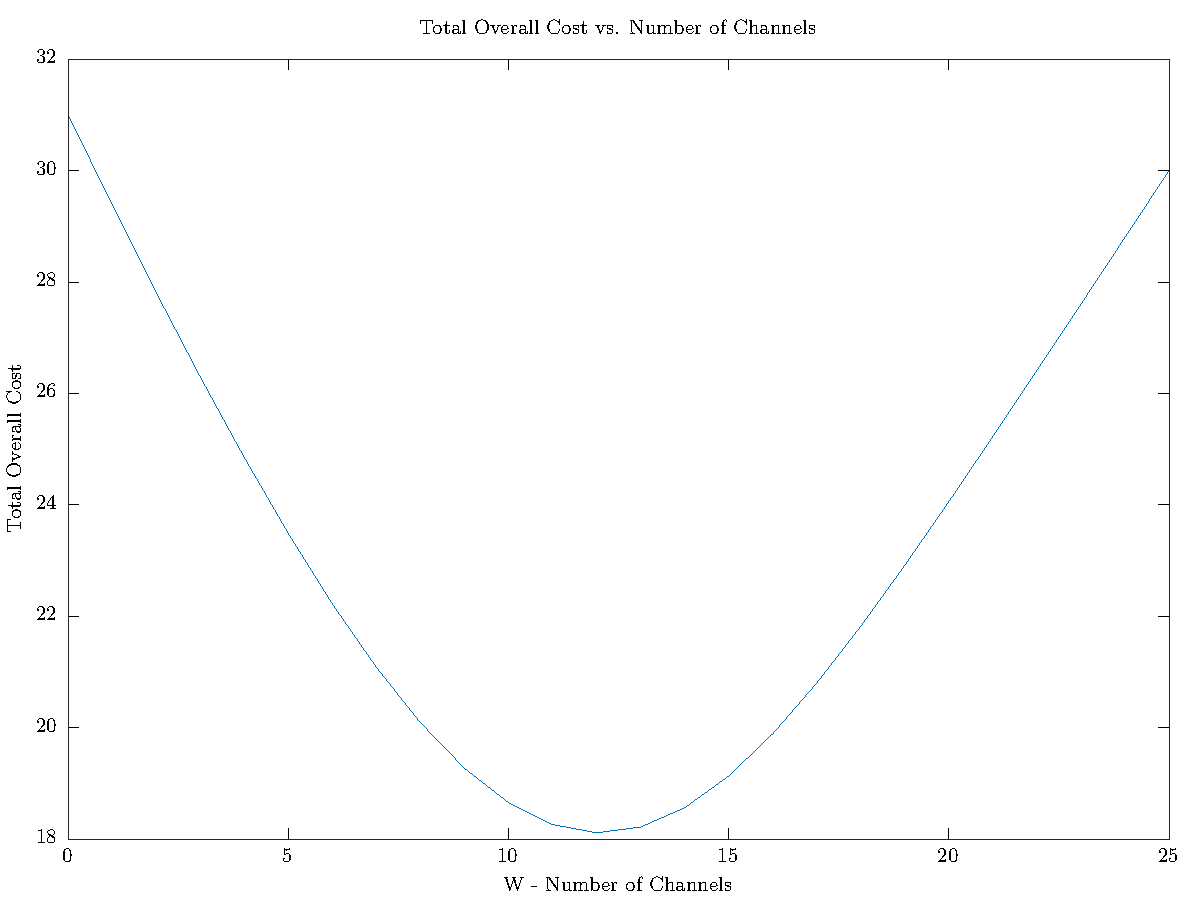
\includegraphics[width=0.8\textwidth]{code/Q5/Q5}
	\caption{Plot of the Total Overall Cost within the given system}
	\label{fig:code-Q5}
\end{figure}

Therefore, the number of channels which minimizes the total overall cost is 12.

The above answers were obtained using the Erlang-B Iterative Formula, programmed
using GNU-Octave. This code is shown below.

\lstinputlisting[language=Octave]{code/Q5/erlang.m}


\section{Question 6}
\subsection{Part 1}

The following figure shows the block diagram of traffic flows/overflows within
the system. The A values ($A_{micA}$, $A_{micB}$, $A_{micC}$, $A_{mac}$, represent the
``Offered Load'' to the cells (Micro Cell A, Micro Cell B, Micro Cell C, Macro
Cell) respectively. $N_{mic}$ represents the number of channels in the micro
cells, while  $N_{mac}$ represents the number of channels in the macro cell. The
``Offered Load'' for the Overflow is represented by $A^*$, with the number of
channels represented by $N_{mac} + N^*$.

\begin{figure}[H]
	\centering
	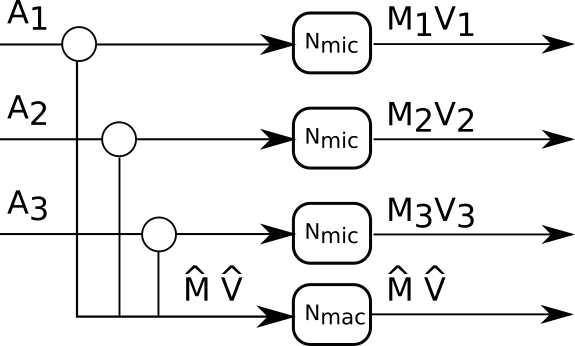
\includegraphics[width=0.8\textwidth]{images/Q6}
	\caption{Traffic Flows/Overflows Block Diagram}
	\label{fig:images-Q6}
\end{figure}

\subsection{Part 2}

The following table shows the Transition Probability Matrix for the process.

\begin{table}[H]
	\centering
	\caption{Transition Probability Matrix}
	\label{tab:label}
	\begin{tabular}{|c|c|c|c|c|c|}
		\hline
		0 & 1 & 2 & 3 & 4 & \ldots \\
		\hline
		0 & 0.5 & 0.5 & 0 & 0 & \ldots \\
		0 & 0 & 0.5 & 0.5 & 0 & \ldots \\
		0 & 0 & 0 & 0.5 & 0.5 & \ldots \\
		0 & 0 & 0 & 0 & 0.5 & 0.5 \\
		\hline
	\end{tabular}
\end{table}

\subsection{Part 3}

The minimum cost of the system is 102 cost units. This cost
corresponds to 24 Micro Cell Channels at 1 cost unit per channel, and 78 Macro
Cell Channels at 3 cost units per channel.

The figure below shows the Total System cost versus the number of Micro Cell
channels. The cost decreases to 102 up to 24 Micro Cell Channels, and increases
past this value.

\begin{figure}[H]
	\centering
	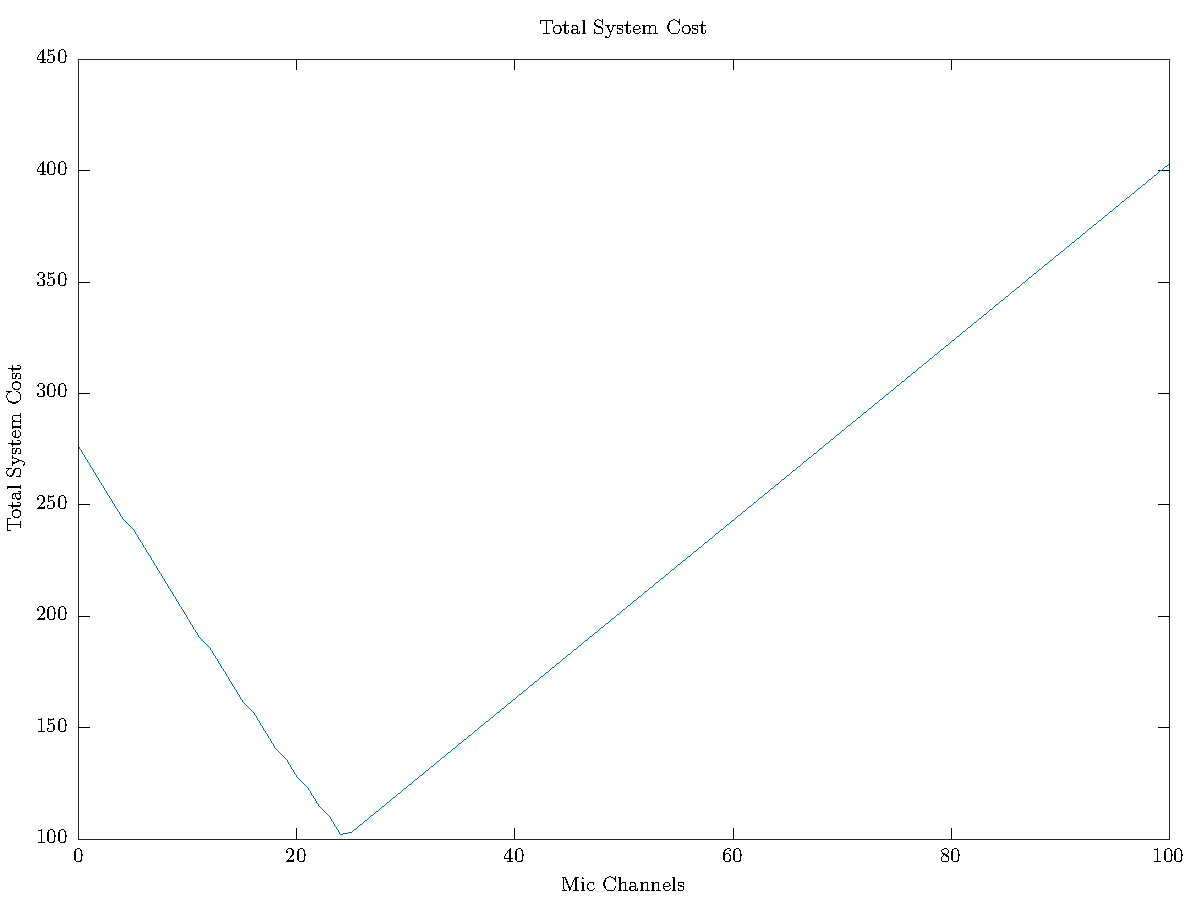
\includegraphics[width=0.8\textwidth]{code/Q6/Q6}
	\caption{Total System Cost vs. Micro Cell Channels}
	\label{fig:code-Q6-Q6}
\end{figure}

The following octave code shows the GNU-Octave implementation of the presented
problem. In order to calculate the minimum cost, the calculations described in
Part 2 are executed for increasing values of Micro Cell and Macro Cell Channels.
The blocking probability of each micro cell is calculated using the loops
current micro cell channel number and each cells respective offered load. These
blocking probabilities can be used to find the mean and variance for each cell.

A nested loop increments through the number of macro cell channels, calculating
the blocking probability, mean, and variance of the directly accessed macro
cell. The offered load and number of channels for the overflow channel is given
by using Rapps approximations on the total means and variances for the micro and
macro cells.

Using the offered load and number of channels for the overflow channel from
Rapps approximations, the overall blocking probability can be calculated. This
loop executes until the blocking probability drops below the required
QoS value of 1%.

For all calculations of blocking probabilities, the iterative method for
Erlang-B is used.

\lstinputlisting[language=octave]{code/Q6/q6.m}

\clearpage
\printbibliography
\end{document}
